\documentclass[10pt,a4paper]{amsart}
\usepackage[margin=19mm]{geometry}
\usepackage{amsmath,amssymb,mathtools}
\usepackage[scr=rsfs,cal=euler]{mathalfa}
\usepackage{xfrac}
\usepackage[unicode,hidelinks,bookmarks=false]{hyperref}
\newcommand{\ie}{i.e.\ }
\newcommand{\cf}{cf.\ }
\newcommand{\resp}{respectively\ }
\newcommand{\Subsection}{\subsection}
\providecommand{\nobreakdash}{\nobreak\hbox{-}}
\setlength{\emergencystretch}{2em}
\multlinegap0pt
\newtheorem{comment}{Comment}
\usepackage{tikz}
\usepackage{bm}
\usepackage{amssymb}
\usepackage{xcolor}
\usepackage{mathtools}
\usepackage{enumerate}
\newtheorem{theorem}{Theorem}
\newtheorem{lemma}{Lemma}
\title{Matchings in the hypercube with specified edges}
\author{Joshua Erde}
\date{Source: arXiv:2404.03950v3 (CC BY 4.0)}
\begin{document}
\maketitle

\noindent\emph{Source and licence.} Matchings in the hypercube with specified edges. Version arXiv:2404.03950v3 (CC BY 4.0), distributed by arXiv under the Creative Commons Attribution 4.0 International licence, http://creativecommons.org/licenses/by/4.0/, as recorded in the arXiv licence metadata for this exact version and shown on the abstract page https://arxiv.org/abs/2404.03950v3. Full licence notice: \texttt{licenses/arxiv-2404.03950-CC-BY-4.0.txt}.\par\smallskip

\noindent\textit{Editorial scope.} Counted unit: the article's theorem t:perfect (source0.tex lines 53--55). The article's complete original proof of it is delivered with it (source0.tex lines 172--283, one \texttt{proof} environment of 112 lines, which the article places away from the statement). No mathematics is written, repaired or re-derived: the statement and the proof are the article's own lines, in the article's own notation, and no retained line is substituted or re-flowed.  Retained uncounted as the source-local context the proof needs: lines 30--32; lines 67--69; lines 154--156.  Nothing was omitted from any retained span, so the package carries no omission record.  No retained line contains a citation, so the wrapper carries no bibliography and no bibliography entry.  The retained lines contain the article's own diagram code, which the wrapper typesets with the standard tikz packages; no image file is delivered and the package declares no asset dependency.  Editorial formatting only, in addition: an AMS \texttt{amsart} preamble that restates the article's own declarations and macros used by the retained lines, namely the environments \texttt{theorem}, \texttt{lemma} on separate counters, together with the standard packages those lines need.  The retained environments print in this document as Theorem 1, Lemma 1 in order of appearance, whereas the article prints the same items with the numbering of its own full document.  The complete native source of the article as distributed in the arXiv e-print for this exact version is bundled unchanged as \texttt{sources/157259/source0.tex}.
\begin{equation}\label{e:null}
\sum_{i=1}^{2^{n-1}} \bm{d_i} = \sum_{i=1}^{2^{n-1}}  \bm{a_i} - \bm{b_i} =   \sum_{i=1}^{2^{n-1}}  \bm{a_i} + \bm{b_i} = \sum_{\bm{v} \in \mathbb{F}_2^n} \bm{v} = \bm{0}.
\end{equation}

\begin{lemma}\label{l:admissible}
If $\bm{x} \in \mathbb{N}^{n}$ is admissible and $x_{n+1} = 2^{n} - 2||\bm{x}||_1$, then $(2\bm{x},x_{n+1})$ is a perfect admissible tuple.
\end{lemma}

\begin{lemma}\label{l:first}
Let $n\geq 2$, and let $\bm{x} \in \mathbb{N}^{n+1}$ be even with $||\bm{x}||_1 \leq 2^{n}$ and $x_{n+1} \geq 2 o(\bm{x})$. If $\bm{y} := \left(\frac{x_1}{2},\frac{x_2}{2}, \ldots, \frac{x_n}{2}\right)$, then there exists a perfect even $\bm{y'} \in \mathbb{N}^n$ such that $\bm{y} \preceq \bm{y'}$
\end{lemma}

\begin{theorem}\label{t:perfect}
Let $n \geq 2$. A perfect tuple $\bm{x} \in \mathbb{N}^n$ is admissible if and only if it is even.
\end{theorem}

\begin{proof}[Proof of Theorem \ref{t:perfect}]
We first note that by \eqref{e:null} every perfect admissible tuple is even.

For the other direction, let us suppose towards a contradiction that the theorem does not hold, and let $\bm{x} \in \mathbb{N}^{n+1}$ be a perfect even tuple which is not admissible, with $n$ as small as possible. Let $\bm{y} = \left(\frac{x_1}{2},\frac{x_2}{2},\ldots, \frac{x_n}{2}\right)$. Note that, $\bm{x} = (2\bm{y},x_{n+1})$ and, since $\bm{x}$ is perfect, $x_{n+1} = 2^n - 2||\bm{y}||_1$. Furthremore, since $\bm{x}$ is not admissible, by Lemma \ref{l:admissible} neither is $\bm{y}$.

If $\bm{x}$ is such that $x_{n+1} \geq 2n$, then since $o(\bm{x}) \leq n$, it follows from Lemma \ref{l:first} that there exists a perfect even $\bm{y'} \succeq \bm{y}$. However, since $\bm{y}$ is not admissible, neither is $\bm{y'} \in \mathbb{N}^n$, contradicting our choice of $\bm{x}$.

Hence, we may assume that $x_{n+1} < 2n$. However, if $n+1 \geq 8$, then since $x_1\leq x_2 \leq \ldots \leq x_{n+1}$,
\begin{equation} \label{e:dim}
x_{n+1} \geq \frac{2^n}{n+1} \geq 2n,
\end{equation}
and hence we may assume that $n+1 \leq 7$.

This reduces the proof to a finite case check, and in fact more precise applications of Lemma \ref{l:first} will deal with all but three of the remaining cases. In the table below we list all perfect even tuples $\bm{x} \in \mathbb{N}^{n+1}$ with $3\leq n+1 \leq 7$ such that $x_{n+1} < 2n$. For tuples listed in blue, $x_{n+1} \geq 2o(\bm{x})$, and so by Lemma \ref{l:first} these tuples cannot be minimal counterexamples. The remaining tuples are listed in red.

\begin{center}
\begin{tabular}{ |c|c| } 
 \hline
 $n+1=3$ & \color{blue}$(0,2,2)$\color{black}  \\ 
 $n+1=4$ &  \color{blue}$(0,0,4,4)$\color{black}, \color{blue}$(0,2,2,4)$\color{black}, \color{red}$(2,2,2,2)$  \\ 
$n+1=5$ &  \color{blue}$(0,0,4,6,6)$\color{black}, \color{blue}$(0,2,2,6,6)$\color{black}, \color{blue}$(0,2,4,4,6)$\color{black},\\
& \color{blue}$(2,2,2,4,6)$\color{black}, \color{blue}$(0,4,4,4,4)$\color{black}, \color{blue}$(2,2,4,4,4)$ \color{black} \\ 
$n+1=6$ &  \color{blue}$(0,0,8,8,8,8)$\color{black},\color{blue}$(0,2,6,8,8,8)$\color{black},\color{blue}$(0,4,4,8,8,8)$\color{black},\color{blue}$(2,2,4,8,8,8)$\color{black}, \\
&\color{blue}$(0,4,6,6,8,8)$\color{black}, \color{blue}$(2,2,6,6,8,8)$\color{black},\color{blue}$(2,4,4,6,8,8)$\color{black},\\
& \color{blue}$(4,4,4,4,8,8)$\color{black},
\color{blue}$(0,6,6,6,6,8)$\color{black}, \color{blue}$(2,4,6,6,6,8)$, \\
& \color{blue}$(4,4,4,6,6,8)$\color{black},
\color{red}$(2,6,6,6,6,6)$\color{black}, \color{blue}$(4,4,6,6,6,6)$\color{black}\\ 
 $n+1=7$ &  \color{blue}$(4,10,10,10,10,10,10)\color{black}$,\color{blue}$(6,8,10,10,10,10,10)$\color{black},\color{blue}$(8,8,8,10,10,10,10)$\color{black}  \\ 
 \hline
\end{tabular}
\end{center}
So, the only three cases we have to construct by hand are $(0,2)$, $(2,2,2,2)$ and $(2,6,6,6,6,6)$. At this point it is slightly easier to apply Lemma \ref{l:admissible} to see that it remains to show that $(1)$, $(1,1,1)$ and $(3,3,3,3,1)$ are admissible, where in fact we show the stronger statement that $(3,3,3,3,3)$ is admissible.

The first is trivial. The second is only slightly less trivial and is given already in Figure \ref{f:3dim}. The third is a fun exercise and one possible solution is given in Figure \ref{f:5dim}.
\begin{comment}
\begin{figure}[!ht]
\centering
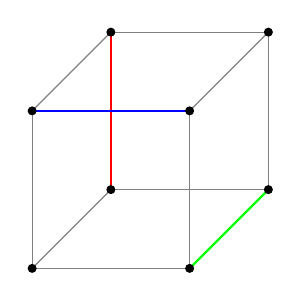
\begin{tikzpicture}[scale=2]

\draw[gray] (0,0)--(1,0)--(1,1)--(0,1)--(0,0);
\draw[gray] (0.5,0.5)--(1.5,0.5)--(1.5,1.5)--(0.5,1.5)--(0.5,0.5);
\draw[gray] (0,0)--(0.5,0.5) (1,1)--(1.5,1.5) (1,0)--(1.5,0.5) (0,1)--(0.5,1.5);

\draw[red,thick] (0.5,0.5)--(0.5,1.5);
\draw[blue,thick] (0,1)--(1,1);
\draw[green,thick] (1,0)--(1.5,0.5);

 \node[shape=circle,draw=black, fill, scale=0.3] at (0,0){};
  \node[shape=circle,draw=black, fill, scale=0.3] at (1,0){};
   \node[shape=circle,draw=black, fill, scale=0.3] at (0,1){};
    \node[shape=circle,draw=black, fill, scale=0.3] at (1,1) {};
     \node[shape=circle,draw=black, fill, scale=0.3] at (0.5,0.5) {};
      \node[shape=circle,draw=black, fill, scale=0.3] at (1.5,0.5) {};
       \node[shape=circle,draw=black, fill, scale=0.3] at (0.5,1.5) {};
        \node[shape=circle,draw=black, fill, scale=0.3] at (1.5,1.5) {};
\end{tikzpicture}
\caption{A matching in $Q^3$ with profile $(1,1,1)$.}\label{f:3dim}
\end{figure}
\end{comment}

\begin{figure}[!ht]
\centering
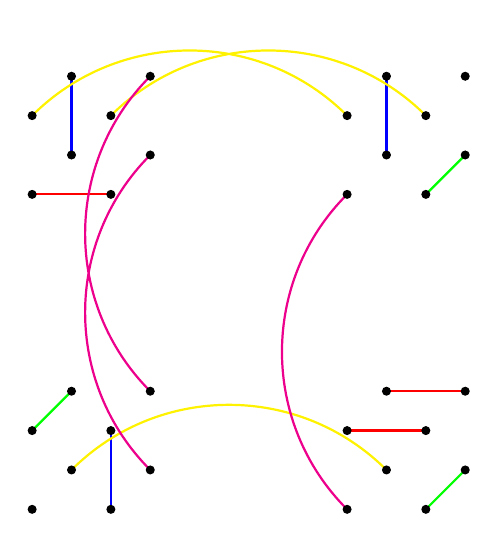
\begin{tikzpicture}

\draw[red,thick] (0,4)--(1,4) (4.5,1.5)--(5.5,1.5) (4,1)--(5,1);
\draw[blue,thick] (1,0)--(1,1) (4.5,4.5)--(4.5,5.5) (0.5,4.5)--(0.5,5.5);
\draw[green,thick] (0,1)--(0.5,1.5) (5,4)--(5.5,4.5) (5,0)--(5.5,0.5);
\draw[yellow,thick] (0.5,0.5) to[out=45,in=135] (4.5,0.5) (1,5) to[out=45,in=135] (5,5) (0,5) to[out=45,in=135] (4,5);
\draw[magenta,thick] (4,0) to[out=135,in=225] (4,4) (1.5,1.5) to[out=135,in=225] (1.5,5.5) (1.5,0.5) to[out=135,in=225] (1.5,4.5);


\node[shape=circle,draw=black, fill, scale=0.3] at (0,0){};
  \node[shape=circle,draw=black, fill, scale=0.3] at (1,0){};
   \node[shape=circle,draw=black, fill, scale=0.3] at (0,1){};
    \node[shape=circle,draw=black, fill, scale=0.3] at (1,1) {};
     \node[shape=circle,draw=black, fill, scale=0.3] at (0.5,0.5) {};
      \node[shape=circle,draw=black, fill, scale=0.3] at (1.5,0.5) {};
       \node[shape=circle,draw=black, fill, scale=0.3] at (0.5,1.5) {};
        \node[shape=circle,draw=black, fill, scale=0.3] at (1.5,1.5) {};

        \node[shape=circle,draw=black, fill, scale=0.3] at (4,0){};
  \node[shape=circle,draw=black, fill, scale=0.3] at (5,0){};
   \node[shape=circle,draw=black, fill, scale=0.3] at (4,1){};
    \node[shape=circle,draw=black, fill, scale=0.3] at (5,1) {};
     \node[shape=circle,draw=black, fill, scale=0.3] at (4.5,0.5) {};
      \node[shape=circle,draw=black, fill, scale=0.3] at (5.5,0.5) {};
       \node[shape=circle,draw=black, fill, scale=0.3] at (4.5,1.5) {};
        \node[shape=circle,draw=black, fill, scale=0.3] at (5.5,1.5) {};

        \node[shape=circle,draw=black, fill, scale=0.3] at (0,4){};
  \node[shape=circle,draw=black, fill, scale=0.3] at (1,4){};
   \node[shape=circle,draw=black, fill, scale=0.3] at (0,5){};
    \node[shape=circle,draw=black, fill, scale=0.3] at (1,5) {};
     \node[shape=circle,draw=black, fill, scale=0.3] at (0.5,4.5) {};
      \node[shape=circle,draw=black, fill, scale=0.3] at (1.5,4.5) {};
       \node[shape=circle,draw=black, fill, scale=0.3] at (0.5,5.5) {};
        \node[shape=circle,draw=black, fill, scale=0.3] at (1.5,5.5) {};

        \node[shape=circle,draw=black, fill, scale=0.3] at (4,4){};
  \node[shape=circle,draw=black, fill, scale=0.3] at (5,4){};
   \node[shape=circle,draw=black, fill, scale=0.3] at (4,5){};
    \node[shape=circle,draw=black, fill, scale=0.3] at (5,5) {};
     \node[shape=circle,draw=black, fill, scale=0.3] at (4.5,4.5) {};
      \node[shape=circle,draw=black, fill, scale=0.3] at (5.5,4.5) {};
       \node[shape=circle,draw=black, fill, scale=0.3] at (4.5,5.5) {};
        \node[shape=circle,draw=black, fill, scale=0.3] at (5.5,5.5) {};

\end{tikzpicture}
\caption{A matching in $Q^5$ with profile $(3,3,3,3,3)$.}\label{f:5dim}
\end{figure}
\end{proof}

\end{document}
